%   % !TEX root = ../../VIII,3_Rahmen-TeX_8-1.tex
%
%
%   Band VIII, 3 N.~??A35
%   Signatur/Tex-Datei: LH_37_04_078
%   RK-Nr. 60239
%   Überschrift: Cohaesio
%   Modul: Mechanik / Festigkeit
%   Datierung: [Ende Januar 1683 bis erste Hälfte 1684 (?)]
%   WZ: (keins)
%   SZ: (keins)
%   Bilddateien (PDF): LH_37_04_078_d (insgesamt: eins)
%
%
\selectlanguage{ngerman}%
\frenchspacing%
%
\begin{ledgroupsized}[r]{120mm}
\footnotesize
\pstart
\noindent\textbf{Überlieferung:}
\pend
\end{ledgroupsized}
\begin{ledgroupsized}[r]{114mm}
\footnotesize
\pstart \parindent -6mm
\makebox[6mm][l]{\textit{L}}%
Aufzeichnung: LH~XXXVII~4 Bl.~78.
Ein Zettel (14 x 5 cm);
Tinte verblasst;
Papiererhaltungsmaßnahmen.
Zwei Seiten. 
\pend
\end{ledgroupsized}
%
%
\vspace*{5mm}
\begin{ledgroup}
\footnotesize 
\pstart
\noindent\textbf{Datierungsgründe:}
In der vorliegenden, der Frage nach dem physikalischen Zusammenhalt der Körper gewidmeten Aufzeichnung N.~16 weist Leibniz (erneut) die in Descartes' \textit{Principia} geäußerte Antwort zurück und knüpft zudem an eine von ihm selbst früher vorgeschlagene Erklärung an, die er jetzt aber ebenfalls ablehnt (S.~\refpassage{LH_37_04_078v_olim_irhv-1}{LH_37_04_078v_olim_irhv-2}).
Als Beleg für diese nunmehr überholte Betrachtungsweise lassen sich Texte aus der Pariser Zeit (Frühjahr 1672 bis Winter 1672/1673) anführen wie etwa \textit{Propositiones quae\-dam physicae} (\textit{LSB} VI,~3 N.~2\textsubscript{3}\cite{00258}) und vornehmlich \textit{De consistentia corporum} (ebd. N.~4\cite{01299}; die genauen Stellenangaben entnehme man den Erläuterungen weiter unten).
Die in diesen Texten belegte Auffassung der Kohäsion bezeichnet Leibniz in N.~16 als eine solche, die er \textit{olim} vertreten habe, d.h. \glqq einst\grqq\ bzw. \glqq vor geraumer Zeit\grqq\ (S.~\refpassage{LH_37_04_078v_olim_irhv-1}{LH_37_04_078v_olim_irhv-2}).
Dies rechtfertigt wohl die Annahme, dass N.~16 nicht vor Leibnizens Rückkehr nach Deutschland Ende 1676 entstand, vermutlich aber noch später.
\pend%
\pstart%
Eine weitere Eingrenzung der Datierung ergibt sich aus der in N.~16 angedeuteten Erklärung der Kohäsion: Der Zusammenhalt zweier Körper rühre vom Druck des umgebenden Mediums her, das im mikroskopischen Bereich, gleich einer \glqq Presse\grqq\ (\textit{praelum}), das Ineinandergreifen der Oberflächen beider Körper zur Folge habe (S.~\refpassage{LH_37_04_078r_causacohaesionis_bfjh-1}{LH_37_04_078r_causacohaesionis_bfjh-2}).
Ein solcher Erklärungsansatz entspricht den Ausführungen über den Ursprung der Kohäsion, die in Texten aus diesem Band wie N.~14\textsubscript{3} \textit{Explicatio mechnica elastri} und N.~14\textsubscript{7} \textit{Demonstratio quod extensiones elasticorum sint viribus tendentibus proportionales} anzutreffen sind (siehe insbesondere N.~14\textsubscript{3}, S.~\refpassage{LH_35_09_16_020v_PresseModell_gscd-1}{LH_35_09_16_020v_PresseModell_gscd-2}).
Diese beiden Texte, die Leibniz im Laufe seiner umfangreichen Untersuchung über die Festigkeit der Balken verfasste, lassen sich insgesamt auf die Zeitspanne zwischen Ende Januar 1683 und der ersten Hälfte 1684 datieren (siehe die editorische Vorbemerkung zum Textkomplex N.~14).
Ihre inhaltliche Verwandtschaft mit N.~16 wird hier als Zeichen für eine gemeinsame Entstehungszeit gedeutet.
Daraus ergibt sich die für die vorliegende Aufzeichnung vorgeschlagene Datierung.
Dass N.~16 vor den Entwürfen N.~14\textsubscript{3} und N.~14\textsubscript{7} verfasst wurde (jedenfalls aber nach Ende 1676), ist unwahrscheinlich, weil die in diesen Texten vertretene neue Auffassung der Kohäsion sich als Ergebnis aus der Untersuchung über die Festigkeit der Balken erweist.
Eine spätere Datierung von N.~16 hingegen ist nach heutigem Kenntnisstand nicht auszuschließen. (Eine ähnliche Ansicht wie in der vorliegenden Aufzeichnung vertritt Leibniz etwa in der \textit{Dynamica}, pars II, sectio III, prop.~20;\cite{01354} \textit{LMG} VI, S.~510\,f.\cite{01043})
\pend 
\end{ledgroup}
%
\selectlanguage{latin}%
\frenchspacing%
%
%
\newpage%
%\vspace{8mm}
\pstart
\noindent
\lbrack78~r\textsuperscript{o}\rbrack\ %%%% Blatt 78r
\pend
\vspace{-0.5em}%
\count\Bfootins=1100
\count\Afootins=1000
\count\Cfootins=1100
\pstart
\centering
{Cohaesio}\protect\index{Sachverzeichnis}{cohaesio}
\pend
% \count\Bfootins=1000
% \count\Cfootins=1000
%
\pstart
\vspace{0.5em}%
\noindent
\edtext{Dicit Cartesius\protect\index{Namensregister}{\textso{Descartes} (Cartesius, des Cartes), René 1596\textendash1650}
\edtext{in Epist.\protect\index{Sachverzeichnis}{epistola}}{%
\lemma{in}\Bfootnote{%
\hspace{-0,5mm}Epist.
\textit{erg.~L}}}
ad Morinum\protect\index{Namensregister}{\textso{Morin} (Morinus), Jean-Baptiste 1583\textendash1656}
se demonstrare posse
id omne in physicis\protect\index{Sachverzeichnis}{physica} esse falsum, 
quod non similitudine\protect\index{Sachverzeichnis}{similitudo rerum sensibilium}
aliqua a rebus sensibilibus\protect\index{Sachverzeichnis}{res sensibilis} sumta illustrari possit.}{%
\lemma{Dicit \lbrack...\rbrack\ possit}\Cfootnote{%
R.~\textsc{Descartes}, Brief an J.-B.~Morin vom 12.\ September 1638\cite{01298}
(\textit{DL} I, Nr.~62, S.~290\,f.;\cite{00209}
\textit{DO} II, Nr.~143, S.~367.21\textendash368.12).\cite{00120}}}
%
Sed qua quaeso similitudine rerum sensibilium\protect\index{Sachverzeichnis}{similitudo rerum sensibilium} illustrabit,
%
\edtext{quod asserit quietem\protect\index{Sachverzeichnis}{quies} unius corporis prope aliud esse gluten\protect\index{Sachverzeichnis}{gluten}
sufficiens quod efficiat ut sine vi separari non possint.}{%
\lemma{quod \lbrack...\rbrack\ possint}\Cfootnote{%
R.~\textsc{Descartes}, \textit{Principia}, pars~II, §~55\cite{00035}
(Amsterdam 1644, S.~62;
\textit{DO} VIII,~1, S.~71.8\textendash10).\cite{00120}}}
%
Mihi
%
\edtext{vero \edlabel{LH_37_04_078r_causacohaesionis_bfjh-1}causa prima connexionis%
\protect\index{Sachverzeichnis}{causa connexionis}\protect\index{Sachverzeichnis}{connexio}
est pressio ambientium,\protect\index{Sachverzeichnis}{pressio ambientium}}{%
\lemma{vero}\Bfootnote{%
\textit{(1)}~gluten
\textit{(2)}~causa prima connexionis est
\textit{(a)}~\textlangle rer\textrangle\
\textit{(b)}~pressio ambientium,%
~\textit{L}}}
%
quod utique sensibilibus exemplis\protect\index{Sachverzeichnis}{exemplum sensibile} illustrari potest.
Et ob hanc fit,
ut corpus quiescens\protect\index{Sachverzeichnis}{corpus quiescens} prope aliud corpus in ipsum
%
\edtext{prematur et ab ambiente\protect\index{Sachverzeichnis}{corpus ambiens} adigatur}{%
\lemma{ipsum}\Bfootnote{%
\textit{(1)}~quod adigatur et
\textit{(2)}~prematur et ab ambiente adigatur%
~\textit{L}}}
%
velut praelo,\protect\index{Sachverzeichnis}{praelum}
cumque nullum sit perfecte durum\protect\index{Sachverzeichnis}{corpus perfecte durum}
aut politum,\protect\index{Sachverzeichnis}{corpus perfecte politum}
ei nonnihil inseritur.\edlabel{LH_37_04_078r_causacohaesionis_bfjh-2}
An autem idem dicendum sit de corporibus perfecte duris et
%
\edtext{politis, dubito.}{%
\lemma{politis,}\Bfootnote{%
\textit{(1)}~nescio
\textit{(2)}~dubito.%
~\textit{L}}}
%
Haec enim nulla sunt.
Ponamus
%
\lbrack78~v\textsuperscript{o}\rbrack\ %%%% 78~v\textsuperscript{o}
%
itaque corpora perfecte dura\protect\index{Sachverzeichnis}{corpus perfecte durum}
%
\edtext{et polita\protect\index{Sachverzeichnis}{corpus perfecte politum}}{%
\lemma{et}\Bfootnote{%
\hspace{-0,5mm}polita
\textit{erg.~L}}}
%
praelo\protect\index{Sachverzeichnis}{praelum} comprimi,
an difficilius quam ante separabuntur?
%
\edtext{Quaero\edlabel{LH_37_04_078v_olim_irhv-1} etiam}{%
\lemma{Quaero}\Bfootnote{%
\textit{(1)}~et
\textit{(2)}~etiam%
~\textit{L}}}
%
si corpus moveatur ita
ut in alterius locum tendat,
simulque ipsum contingat,
%
\edtext{\lbrack an\rbrack}{%
\lemma{an}\Bfootnote{\textit{erg. \mbox{Hrsg.}}}}
%
inde sequatur
%
\edtext{cohaesio,\protect\index{Sachverzeichnis}{cohaesio}
\edtext{ita\hspace{0.1mm} olim\hspace{0.1mm} credebam,\hspace{0.1mm}}{%
\lemma{ita olim credebam}\Cfootnote{%
\selectlanguage{german}{Siehe etwa G.\,W. \textsc{Leibniz}, \textit{De consistentia corporum} (\textit{LSB} VI,~3 N.~4, bes. S.~95.25\textendash96.11\cite{01299}).
Dieser auf die Zeitspanne vom Herbst 1672 bis zum Winter 1672/1673 datierbare Entwurf hängt mit weiteren naturphilosophischen Texten aus der frühen Pariser Zeit zusammen; vgl. etwa \textsc{Ders.}, \textit{Propositiones quaedam physicae}, Dritter Entwurf, prop. 24 (ebd. N.~2\textsubscript{3}, S.~42.20\textendash47.22\cite{00258}).}}}
sed\hspace{0.1mm} jam\hspace{0.1mm} video\hspace{0.1mm}}{%
\lemma{cohaesio,}\Bfootnote{%
\textit{(1)}~sed jam video id op\textlangle or\textrangle\
\textit{(2)}~ita olim \lbrack...\rbrack\ jam video%
~\textit{L}}}\hspace{0.1mm}
%
contrarium\hspace{0.1mm} esse\hspace{0.1mm} verius. \hspace{0.1mm}\edlabel{LH_37_04_078v_olim_irhv-2}
Moveatur\hspace{0.1mm} enim \hspace{0.1mm}\textit{ab} \hspace{0.1mm}secundum
\pend
  \vspace{1.2em}%
  \centerline{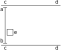
\includegraphics[width=0.32\textwidth]{gesamttex/edit_VIII,3/images/LH_37_04_078_d.pdf}}%
  \vspace{0.5em}%
  \centerline{\lbrack\textit{Fig.~1}\rbrack}%
  \label{LH_37_04_078v_Fig.1}%
  \newpage
\pstart
\noindent \textit{cd}
et secum propellat \textit{e}; 
poterit tamen interea corpus \textit{e}\protect\index{Sachverzeichnis}{corpus propulsum}
incedere secundum lineam \textit{ab}
nec
%
\edtext{ideo difficilius}{%
\lemma{ideo}\Bfootnote{%
\textit{(1)}~celerius
\textit{(2)}~difficilius%
~\textit{L}}}
%
ad hunc motum incitabitur,
aut facilius ad quietem\protect\index{Sachverzeichnis}{quies} redigetur
quam si quiesceret
\textit{ba},
nisi forte ob rationem praeli,\protect\index{Sachverzeichnis}{praelum}
dum \textit{ab} in \textit{e} conatum exercens,\protect\index{Sachverzeichnis}{conatus exercitus}
nonnullas suas eminentias\protect\index{Sachverzeichnis}{eminentia}
eius cavitatibus\protect\index{Sachverzeichnis}{cavitas} altius inserit.
\pend
%\vspace*{-5mm}
%
%
 % \newpage
  \count\Bfootins=1200
\count\Afootins=1200
\count\Cfootins=1200
%  \vspace{1.5em}%
%
%
% \begin{center}
% \includegraphics[width=0.4\textwidth]{gesamttex/edit_VIII,3/images/LH037,04_078v-d.pdf}
% \newline
% [\textit{Fig. 1}]
% \end{center}
%
%
% Ende des Stücks auf S. 78v.